
\section{Spheres with only rational coordinates}
\label{sec:rational}

\begin{figure}
	\begin{center}
		\includegraphics[width=10cm]{Figures/3-bin-generation.pdf}
		\caption{Dividing augmented packing $P$ into three unit bin packings $B_1,B_2,B_3$}
		\label{fig:partition-img-3bins}
	\end{center}
	
\end{figure}


As discussed earlier, for the geometric knapsack
problem with circles or $d$-dimensional hyperspheres, it is not clear
that there always exists an optimal or $(1+\eps)$-approximate solution
that uses only rational coordinates.

We show that for arbitrary dimension, there is a polynomial time $3$-approximation
algorithm  that outputs a solution with rational coordinates only (with
a polynomial number of bits). In particular, this implies that there \emph{exists}
always a solutions with
rational coordinates that is by at most a factor $3$ worse than
the optimal solution with arbitrary coordinates.


\begin{theorem}[$\star$]
	Let $d\in\mathbb{N}$ be a constant. For the geometric knapsack problem
	with $d$-dimensional hyperspheres, there is a polynomial time $3$-approximation
	algorithm.
\end{theorem}


\noindent \emph{Proof sketch.} We first begin with a packing $P$ in the augmented hypercube of dimensions $(1+\eps)\times 1 ...\times 1$ such that the total packed profit is at least $w(\OPT)$, by using \Cref{extended-wowa}. Any hypersphere in the hypercube with diameter \(\geqslant 1-\eps\), we call as huge hypersphere and further prove that there can be atmost one huge hypersphere in any feasible packing. This property essentially helps us to partition the hyperspheres in the bin into three types of hypersphers depending upon their relative position with respect to $\eps$-augmenting planes $\ell$ and $\ell'$ which are perpendicular to the augmented side of the hypercube of length $1+\eps$ and are at a distance of $\eps$ from the left face and right face, respectively (see \Cref{fig:partition-img-3bins}). We pack these three types of hyperspheres in three separate unit hypercube and return the one of maximum weight with weight at least \(\frac{w(\OPT)}{3}\). Details of this result can be found in \Cref{sec:appendix-3-apx}.


\begin{figure}
	\begin{center}
		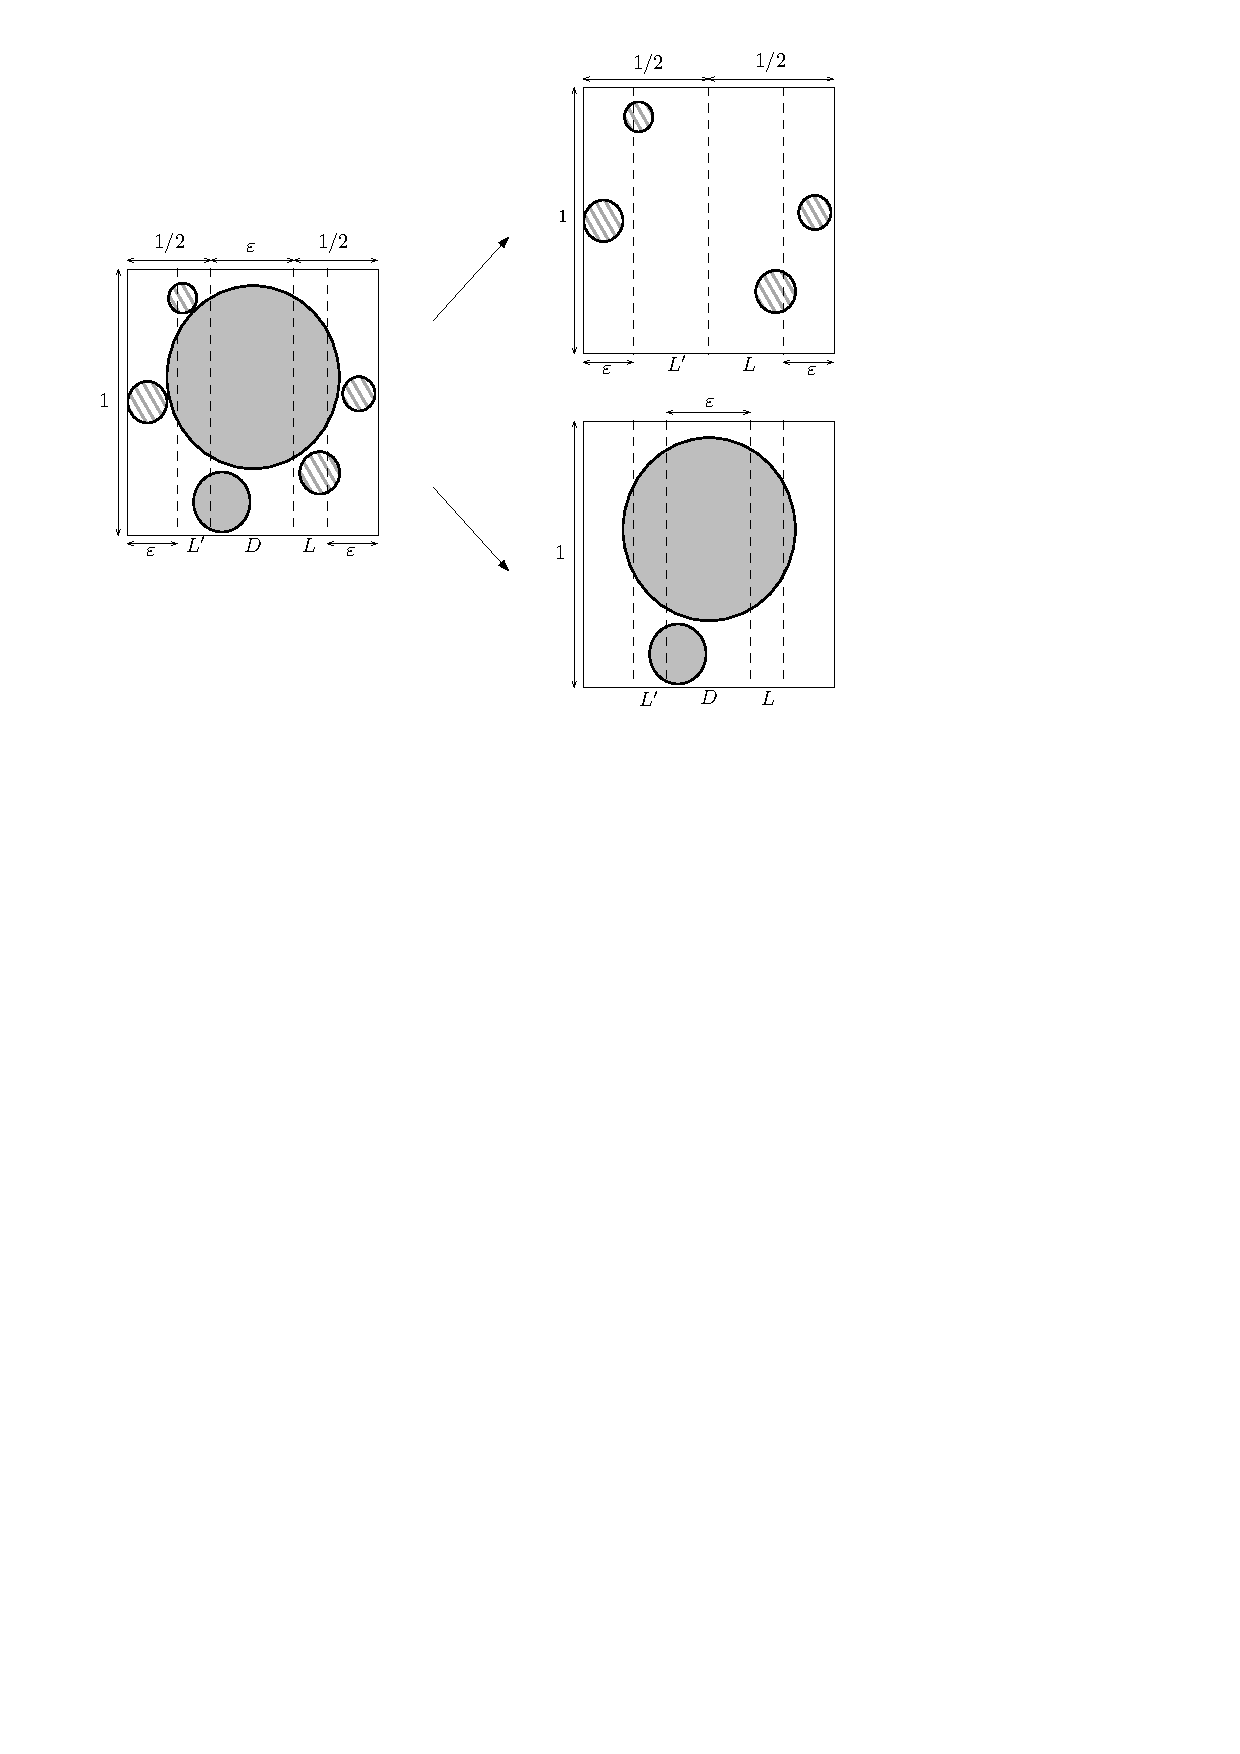
\includegraphics[width=10cm]{Figures/hypersphere_bin_generation.pdf}
		\caption{Dividing augmented packing $P$ into two unit bin packings $B_1$ and $B_2$ with the help of $\eps$-slab $D$}
		\label{fig:partition-img-2bins}
	\end{center}
	
\end{figure}


We improve upon it for any dimension
$d\leqslant8$, to give a $2+\eps$-approximation
algorithm (again, using only rational coordinates with a polynomially bounded number of bits).
\begin{restatable}[\emph{$\star$}]{theorem}{geometricknapsacktheoremapx}
	\label{geometric-knapsack-theorem}
	Let $d\leqslant8$ be a constant. For the geometric knapsack problem with $d$-dimensional hyperspheres, there is a polynomial time $(2+\eps)$-approximation algorithm.
\end{restatable}

\noindent \emph{Proof sketch.} For dimension \(d \leqslant 8\), we show that we do not need to pack huge hypersphere in a separate bin. In case there is no huge hypersphere in our packing, we can partition the set of hyperspheres in two separate bins. In the case there is a huge hypersphere, we prove the existence of a empty \(\eps\)-strip in the middle of the bin which restricts the dimension to \(d \leqslant 8\). This
empty \(\eps\)-strip we can merge the hypersphers in bin $B_1$ and $B_3$ (see \Cref{fig:partition-img-3bins}) in a bin $B_1$  (see \Cref{fig:partition-img-2bins}) and all the packed hyperspheres can be packed in two unit hypercubes. We return the best of the two packings which ensure a profit of \(\frac{(1-\eps)}{2}w(\OPT)\).
Details of this result can be found in \Cref{sec:appendix-2-apx}.
